\documentclass[a4paper]{article}
\usepackage[fontsize=13pt]{scrextend}
\usepackage[utf8]{vietnam}
\usepackage{amsmath}
\usepackage{amsfonts}
\usepackage{xcolor}
\usepackage{titlesec}
\usepackage{mdframed}
\usepackage{amssymb}
\usepackage{pgf,tikz,pgfplots}
\usepackage{graphicx}
\graphicspath{ {figures/} }
\usepackage{array}
\usepackage{cases}
\usepackage{listings}
\usepackage{tabulary}
\usepackage{color}
\usepackage{float} 
\usepackage{hyperref}
\usepackage{multirow}
\usepackage{minitoc}
\pgfplotsset{compat=1.5}
\usepackage{mathrsfs}
\usetikzlibrary{arrows, calc}
\usepackage{fancyhdr}
\usepackage{longtable}
\usepackage{verbatim}

\pagestyle{fancy}
\pagestyle{empty}
\definecolor{dkgreen}{rgb}{0,0.6,0}
\definecolor{gray}{rgb}{0.5,0.5,0.5}
\definecolor{mauve}{rgb}{0.58,0,0.82}
\lstset{frame=tb,
  language=Python,
  aboveskip=3mm,
  belowskip=3mm,
  showstringspaces=false,
  columns=flexible,
  basicstyle={\small\ttfamily},
  numbers=none,
  numberstyle=\tiny\color{gray},
  keywordstyle=\color{blue},
  commentstyle=\color{dkgreen},
  stringstyle=\color{mauve},
  breaklines=true,
  breakatwhitespace=true,
  tabsize=3
}
\hypersetup{
    colorlinks=true,
    linkcolor=blue,
    filecolor=magenta,      
    urlcolor=red,
    pdftitle={An Example},
	% pdfpagemode=FullScreen,
    }
\renewcommand{\listfigurename}{Danh sách hình}
\renewcommand{\listtablename}{Tables}
\newcommand{\tabitem}{~~\llap{\textbullet}~~}
\usepackage[left=2cm,right=2cm,top=2cm,bottom=2cm]{geometry}
\author{Nguyễn Văn Lộc}
\newmdenv[linecolor=black,skipabove=\topsep,skipbelow=\topsep,
leftmargin=-5pt,rightmargin=-5pt,
innerleftmargin=5pt,innerrightmargin=5pt]{mybox}
\fancyhf{}
\lhead{Báo cáo đồ án Mạng máy tính}
\chead{}
\rhead{}
\cfoot{\thepage}
\rfoot{}
\lfoot{}
\pagestyle{fancy}
\renewcommand{\headrulewidth}{0pt}
\renewcommand{\footrulewidth}{0pt}
\begin{document}
\begin{titlepage}
\begin{mybox}
\begin{center}
\fontsize{12}{12}\selectfont
\textbf{ĐẠI HỌC QUỐC GIA THÀNH PHỐ HỒ CHÍ MINH}\\
\textbf{TRƯỜNG ĐẠI HỌC KHOA HỌC TỰ NHIÊN}\\
\textbf{KHOA CÔNG NGHỆ THÔNG TIN}
\end{center}
\vskip 1 cm
\begin{figure}[H]
\begin{center}

\includegraphics[scale=0.25]{figures/logo}
\end{center}
\end{figure}
\vskip 1 cm
\begin{center}
\fontsize{18}{14}\selectfont
\textbf{SƯU LIỆU ĐỒ ÁN MÔN HỌC}\\
\fontsize{26}{16}\selectfont
\textbf{MẠNG MÁY TÍNH}\\
\fontsize{18}{12}\selectfont
\textbf{ĐỀ TÀI: Điều khiển máy tính thông qua email}
\end{center}
\vskip 1 cm
\fontsize{14}{12}\selectfont
\textbf{Giảng viên lý thuyết:} Thầy Đỗ Hoàng Cường\\
\textbf{Lớp:} 20TN\\
\textbf{Thành viên thực hiện:}
\begin{itemize}
\item 20120131 $-$ Nguyễn Văn Lộc
\item 20120536 $-$ Võ Trọng Nghĩa
\item 20120572 $-$ Nguyễn Kiều Minh Tâm
\end{itemize}
\vskip 3 cm
\begin{center}
\textbf{THÀNH PHỐ HỒ CHÍ MINH, THÁNG 5-6 NĂM 2022}
\end{center}
\end{mybox}
\end{titlepage}

\tableofcontents
\listoffigures
\listoftables
\newpage

\section{Giới thiệu}
Ứng dụng cho phép người dùng điều khiển các máy tính (tối đa 4 máy) trong cùng mạng LAN với server. Các chức năng được xây dựng trong đồ án bao gồm:
\begin{itemize}
\item Đăng ký email ứng với IP.
\item Liệt kê danh sách các IP đang kết nối.
\item Ngắt kết nối với một IP.
\item Liệt kê danh sách các tiến trình (process), ứng dụng (application), tắt (kill) một tiến trình.
\item Video màn hình hiện tại.
\item Video webcam hiện tại.
\item Bắt phím nhấn (keylog).
\item Tắt máy, đăng xuất, khởi động lại máy tính.
\item Danh sách các registry, cập nhật giá trị 1 entry trong registry.
\item Liệt kê các thư mục/file trong 1 đường dẫn, copy file.
\end{itemize}
\section{Tổ chức thư mục của chương trình}
Chương trình được tổ chức như sau.
Ở server:
\begin{figure}[H]
\centering{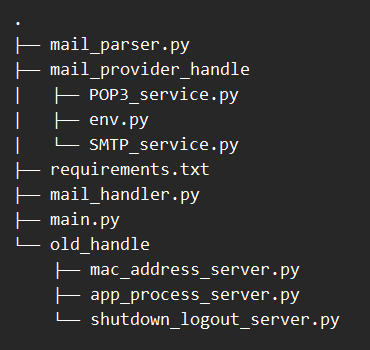
\includegraphics[scale=1]{server_dir}}
\caption{Tổ chức thư mục ở server}
\end{figure}
Server có thư mục \textbf{mail$\mathbf{\_}$provider$\mathbf{\_}$handle} chứa các module phục vụ cho quá trình gửi và nhận mail, thư mục \textbf{old$\mathbf{\_}$handle} chứa một vài hàm được cung cấp sẵn cho quá trình xử lý các yêu cầu. \\
Module \textbf{mail$\mathbf{\_}$parser.py} chứa hàm phục vụ cho quá trình phân tích lệnh được nhận từ email. Module \textbf{mail$\mathbf{\_}$handler} chứa các hàm xử lý yêu cầu, giao tiếp với client và trả kết quả. \\
Tập tin \textbf{requirements.txt} chứa các yêu cầu cần thiết (bên cạnh Python 3.9 trở lên) để chạy chương trình.\\
Tập tin \textbf{main.py} là tập tin chính của server, ta cần chạy tập tin này để khởi động server. \textbf{Lưu ý} khi chạy tập tin này, ta cần thay đổi giá trị \textbf{MAX$\mathbf{\_}$CONNECTION} ở dòng 13 thành giá trị \textbf{bằng đúng} với số lượng client (tối đa 4).
Ở client:
\begin{figure}[H]
\centering{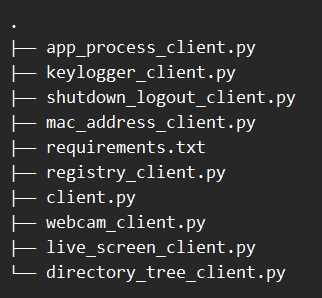
\includegraphics[scale=1]{victim_dir}}
\caption{Tổ chức thư mục ở client}
\end{figure}
Tập tin \textbf{requirements.txt} chứa các yêu cầu cần thiết (bên cạnh Python 3.9 trở lên) để chạy chương trình.\\
Trừ tập tin \textbf{client.py}, các tập tin mã nguồn Python còn lại chứa các hàm xử lý các yêu cầu được gửi đến từ server.\\
Tập tin \textbf{client} là tập tin chính của client, ta cần chạy tập tin này để khởi động client. \textbf{Lưu ý} khi chạy tập tin này ta cần thay đổi giá trị 127.0.0.1 ở dòng 60 thành một giá trị thích hợp.\\
\textbf{Tất cả các client phải được kết nối đến server TRƯỚC khi server bắt đầu nhận và xử lý các lệnh từ email.}


\section{Cú pháp email}
Các email điều khiển được gửi về địa chỉ \textbf{notabotbytheway@outlook.com}.\\ 
Các lệnh phải được viết ở \textbf{tiêu đề} của email.\\
Giá trị key là \textbf{ABDCFE123465}.\\
Cú pháp của các lệnh điều khiển được liệt kê bên dưới:
\begin{itemize}
\item \textbf{AUTH} <key> <IP>: "đăng ký" địa chỉ email để điều khiển <IP>. Tại một thời điểm, mỗi địa chỉ email đăng ký \textbf{duy nhất} với một địa chỉ IP và ngược lại.
\item \textbf{LIST} <key>: liệt kê danh sách các IP đang kết nối.
\item \textbf{DISC}: ngắt kết nối địa chỉ email này với IP hiện tại.
\item \textbf{LIST}$\_$\textbf{PROC}: liệt kê danh sách các tiến trình (process).
\item \textbf{LIST}$\_$\textbf{APP}: liệt kê danh sách các ứng dụng (application).
\item \textbf{KILL} <ID/PID>: tắt (kill) tiến trình có mã là <ID/PID>.
\item \textbf{SCREENSHOT} <time>: chụp màn hình liên tục trong thời gian <time> giây, mặc định là $0.5$ giây.
\item \textbf{WEB}/\textbf{REC} <time>: quay lại webcam của máy trong thời gian <time> giây, mặc định là $5$ giây. 
\item \textbf{KEYLOG} <time>: bắt các phím nhấn trong thời gian <time> giây, mặc định là $10$ giây.
\item \textbf{SHUTDOWN}: tắt máy tính.
\item \textbf{LOGOUT}: đăng xuất. % khỏi Trái Đất
\item \textbf{RESTART}: khởi động lại máy tính.
\item \textbf{MAC}: lấy địa chỉ MAC.
\item \textbf{REGISTRY} \textbf{LIST} <path>: danh sách các registry trong path.
\item \textbf{REGISTRY} \textbf{UPDATE} <registry path> <value> <data type>: cập nhật giá trị của <registry path> thành <value> với kiểu <data type>. <value> \textbf{không} được có khoảng trắng. <data type> được lấy từ \href{https://docs.microsoft.com/en-us/windows/win32/sysinfo/registry-value-types}{link}.
\item \textbf{DIR} \textbf{LIST} <path>: liệt kê các thư mục/file trong đường dẫn <path>.
\item \textbf{DIR} \textbf{COPY} <source file> <destination path>: copy file có tên <source file> đến đường dẫn <destination path>.
\end{itemize}
\section{Gửi và nhận email}
\subsection{Nhận mail}
\begin{itemize}
\item Giao thức sử dụng: POP3.
\item Nhà cung cấp mail: Microsoft Outlook.
\item Sử dụng đa luồng để tối ưu hóa tác vụ.
\end{itemize}
Các hàm sử dụng cho quá trình nhận mail (POP3$\_$service.py):
\begin{lstlisting}
def get_mails():
\end{lstlisting}
Chức năng: Lấy toàn bộ mail đang có trong mail box, tách lấy \textit{email người gửi}, \textit{tiêu đề} và \textit{nội dung} (nếu có), đưa vào hàng đợi để luồng khác xử lý, sau đó thì xóa mail để đảm bảo không trùng lắp với thư cũ.\\
Quá trình thực hiện:
\begin{itemize}
 \item Tạo kết nối POP3 tới server (có sử dụng SSL).
 \item Gửi username (mail) và password để xác thực.
 \item Lấy số lượng mail hiện có qua lệnh \lstinline{LIST}.
 \item Lấy thông tin từng thư qua lệnh \lstinline{RETR}.
 \item Tách lấy thông tin.
 \item Xóa thư với lệnh \lstinline{DELE}.
 \item Gửi lệnh \lstinline{QUIT} ngắt kết nối.
\end{itemize} 

\begin{lstlisting}
def loop():
\end{lstlisting}
Chức năng: Do tính chất của POP3 không cập nhật thư mới, cần phải reload lại sau một khoảng thời gian, nên hàm này sẽ thực hiện việc lấy thư liên tục (gọi tới hàm \lstinline{get_mails()}) khi chương trình khởi chạy.

\subsection{Gửi mail}
\begin{itemize}
\item Giao thức sử dụng: SMTP.
\item Nhà cung cấp mail: Microsoft Outlook.
\item Sử dụng đa luồng để tối ưu hóa tác vụ.
\end{itemize}
Các hàm sử dụng cho quá trình gửi mail (SMTP$\_$service.py):
\begin{lstlisting}
def send(to_: str, subject_: str, content_, file_name):
\end{lstlisting}
Chức năng: Gửi thư đến địa chỉ \lstinline{to_}, với tiêu đề \lstinline{subject_}, nội dung \lstinline{content_} và tên file \lstinline{file_name} nếu nội dung cần gửi là file (file ảnh, video...)\\
Tham số: 
\begin{itemize}
\item \lstinline{ to_}: kiểu \lstinline{str}, là địa chỉ mail người nhận (ví dụ \lstinline{abc@gmail.com}).
\item \lstinline{subject_}: kiểu \lstinline{str}, là tiêu đề của mail.
\item \lstinline{content_}: kiểu \lstinline{str} hoặc \lstinline{bytes}. Nếu là \lstinline{str}, thực hiện gửi như văn bản bình thường. Nếu là  \lstinline{bytes}, gửi như một file với tên file là \lstinline{file_name}.
\item \lstinline{file_name}: kiểu \lstinline{str}, tên file (mặc định là "x.txt").
\end{itemize}
Quá trình thực hiện:
\begin{itemize}
\item Tạo kết nối SMTP tới server (có sử dụng TLS) .
\item Gửi username (mail) và password để xác thực.
\item Soạn thư với định dạng \href{https://datatracker.ietf.org/doc/html/rfc1341}{MIME multipart}.
\item Nếu thư kiểu text, attach \lstinline{MIME text}.
\item Nếu thư kiểu bytes, attach \lstinline{MIME application} với tên file.
\item Gửi payload đến server và đóng kết nối.
\end{itemize}

\begin{lstlisting}
def safe_send(to_:str, subject_:str, content_, file_name):
\end{lstlisting}
Chức năng: Là wrapper cho hàm \lstinline{send}, thực hiện xử lý ngoại lệ: thực hiện gửi thư lại cho đến khi thành công (do trong một số trường hợp, gửi mail quá nhanh server sẽ từ chối nên phải thực hiện lại).\\
Tham số: tương tự \lstinline{send}.

\begin{lstlisting}
def send_threading(to_:str, subject_:str, content_, file_name = "x.txt"):
\end{lstlisting}
Chức năng: tạo threading để gửi thư, các tham số sẽ truyền trực tiếp vào cho hàm \lstinline{safe_send}. (Đây là hàm sẽ được gọi để gửi thư khi được import)\\

\section{Các hàm xử lý yêu cầu}
\subsection{Phân tích câu lệnh}
Hàm phân tích câu lệnh được định nghĩa là:
\begin{lstlisting}
def command_parser(message, sender_address):
\end{lstlisting}
Chức năng: phân tích câu lệnh được gửi đến, gọi hàm tương ứng với yêu cầu của câu lệnh.\\
Tham số:
\begin{itemize}
\item \lstinline{message}: câu lệnh được gửi đến
\item \lstinline{sender_address}: địa chỉ email của người gửi.
\end{itemize}
Không có giá trị trả về.\\

Hàm \lstinline{get_corresponding_ip}
\begin{lstlisting}
def get_corresponding_ip(sender_address):
\end{lstlisting}
Chưc năng: lấy ra địa chỉ IP tương ứng với \lstinline{sender_address}.\\
Tham số:
\begin{itemize}
\item \lstinline{sender_address}: địa chỉ email của người gửi.
\end{itemize}
Trả về địa chỉ IP tương ứng, trả về None nếu không tồn tại.
\subsection{Module mail$\_$handler}
Các hàm được định nghĩa trong module handle.py được sử dụng để xử lý các yêu cầu từ người dùng.
\begin{lstlisting}
def authorize(email, ip):
\end{lstlisting}
Chức năng: authorize địa chỉ email với IP tương ứng.\\
Thám số: 
\begin{itemize}
\item \lstinline{email}: địa chỉ email.
\item \lstinline{ip}: kiểu tuple(str, int) chứa địa chỉ ip và port của client gửi tới.
\end{itemize}
Trả về True nếu thành công, False nếu không thành công.

\begin{lstlisting}
def list_ip():
\end{lstlisting}
Chức năng: trả về danh sách các địa chỉ IP đang được kết nối.

\begin{lstlisting}
def disconnect(email):
\end{lstlisting}
Chức năng: disconnect địa chỉ email hiện tại với IP tương ứng.
Tham số:
\begin{itemize}
\item \lstinline{email}: địa chỉ IP tương ứng.
\end{itemize}
Không có giá trị trả về.

\begin{lstlisting}
def find_corresponding_email(ip_address):
\end{lstlisting}
Chức năng: tìm địa chỉ email tương ứng với IP được truyền vào.
Tham số:
\begin{itemize}
\item \lstinline{ip_address}: kiểu tuple(str, int) chứa địa chỉ ip và port của client gửi tới.
\end{itemize}
Trả về: địa chỉ email tương ứng đang điều khiển địa chỉ IP này.

\begin{lstlisting}
def delete_ip_from_list(ip_address):
\end{lstlisting}
Chức năng: xóa địa chỉ IP ra khỏi danh sách IP kết nối.
Tham số: 
\begin{itemize}
\item \lstinline{ip_address}: kiểu tuple(str, int) chứa địa chỉ ip và port của client gửi tới.
\end{itemize}
Không có giá trị trả về.

\begin{lstlisting}
def remove_this_connection(conn, ip_address):
\end{lstlisting}
Chức năng: loại bỏ kết nối tương ứng với IP.
Tham số:
\begin{itemize}
\item \lstinline{conn}: socket tương ứng.
\item \lstinline{ip_address}: kiểu tuple(str, int) chứa địa chỉ ip và port của client gửi tới.
\end{itemize}
Không có giá trị trả về.

\begin{lstlisting}
def __init__():
\end{lstlisting}
Chức năng: khởi tạo những giá trị liên quan.
\subsection{Process/Application}
Server sẽ gửi lệnh \textbf{APP$\_$PRO} đến client, sau đó sẽ gửi số tương ứng với lệnh.
\begin{itemize}
\item Gửi số 1 nếu ta cần đưa ra danh sách process/application. Sau đó gửi message là \textbf{APPLICATION} hoặc \textbf{PROCESS} tương ứng với yêu cầu của lệnh đến client. Client nhận thông điệp rồi gửi lại danh sách application/process dưới dạng một data frame.
\item Gửi số 0 nếu ta cần kill một process/application. Sau đó ta sẽ gửi ID/PID của đối tượng cần kill. Client nhận thông điệp rồi gửi thông tin về quá trình kill lại cho server.
\end{itemize}
Các hàm cho quá trình này như sau:\\
\begin{itemize}
\item Ở server (mail$\_$handler.py, app$\_$process$\_$server.py):
\begin{lstlisting}
def list_process(ip_address):
\end{lstlisting}
Chức năng: gửi yêu cầu đến client, nhận kết quả rồi gửi mail lại cho người dùng.\\
Tham số: 
\begin{itemize}
\item \lstinline{ip_address}: kiểu tuple(str, int) chứa địa chỉ ip và port của client gửi tới.
\end{itemize}
Trả về: Không có giá trị trả về.
\begin{lstlisting}
def _list(conn:socket.socket, s):
\end{lstlisting}
Chức năng: gửi yêu cầu danh sách tiến trình/ứng dụng đến client, nhận kết quả từ client.\\
Tham số: 
\begin{itemize}
\item \lstinline{conn}: socket kết nối server với client.
\item \lstinline{s}: chuỗi, có giá trị là \textbf{PROCESS} hoặc \textbf{APPLICATION}, thể hiện yêu cầu gửi danh sách tiến trình hoặc ứng dụng.
\end{itemize}
Trả về: Danh sách tiến trình/ứng dụng ở dạng chuỗi.
\begin{lstlisting}

def send_kill(conn:socket.socket, process_id): 
\end{lstlisting}
Chức năng: gửi yêu cầu tắt một tiến trình.\\
Tham số: 
\begin{itemize}
\item \lstinline{conn}: socket kết nối server với client.
\item \lstinline{process_id}: id của tiến trình cần tắt.
\end{itemize}
Trả về: kết quả kill thành công/không thành công.\\
Thư viện sử dụng: pickle, struct, pandas.
\item Ở client (app$\_$process$\_$client.py):
\begin{lstlisting}
def app_process(client):
\end{lstlisting}
Chức năng: nhận yêu cầu từ server, xử lý yêu cầu rồi gửi lại kết quả tương ứng. \\
Tham số: 
\begin{itemize}
\item \lstinline{client}: socket kết nối server với client.
\end{itemize}
Trả về: Không có giá trị trả về.\\
Thư viện sử dụng: pickle, psutil, struct, os, subprocess.\\
Bên cạnh đó, server còn có các hàm (được cung cấp sẵn) phụ trách việc nhận dữ liệu:
\begin{lstlisting}
def recvall(sock, size):
def receive(client):
\end{lstlisting}
Ngoài ra, client còn có các hàm (được cung cấp sẵn) phục vụ việc gửi dữ liệu cho server và xử lý các yêu cầu về application/process trên máy.
\begin{lstlisting}
def send_data(client, data):
def list_apps():
def list_processes():
def kill(pid):
\end{lstlisting}
\end{itemize}






\subsection{Chụp màn hình}
Server sẽ gửi lệnh \textbf{LIVESCREEN} đến client, sau đó sẽ gửi lệnh tương ứng với thời gian cần chụp màn hình, thời gian mặc định là $0.5$ giây. Thời gian chụp không nên quá nhiều, vì giới hạn dung lượng tệp đính kèm trong email. Sau đó, server sẽ nhận ảnh gửi từ client, tạo thành một video.\\
Các hàm cho quá trình này như sau:
\begin{itemize}
\item Ở server (mail$\_$handler.py):
\begin{lstlisting}
def capture_screen(ip_address, time=0.5):
\end{lstlisting}
Chức năng: gửi yêu cầu chụp màn hình đến cho client, nhận hình ảnh từ client gửi lại, tạo video, gửi mail trả lời cho người dùng.\\
Tham số: 
\begin{itemize}
\item \lstinline{ip_address}: kiểu tuple(str, int) chứa địa chỉ ip và port của client gửi tới.
\item \lstinline{time}: thời gian chụp màn hình (giây).
\end{itemize}
Không có giá trị trả về. 
\item Ở client:
\begin{lstlisting}
def capture_screen(client):
\end{lstlisting}
Chức năng: nhận yêu cầu chụp màn hình từ server, chụp màn hình liên tục rồi gửi từng ảnh lại cho server.\\
Tham số: 
\begin{itemize}
\item \lstinline{client}: socket kết nối server với client.
\end{itemize}
Không có giá trị trả về.\\
Thư viện sử dụng: ImageGrab, io, time.\\
Ngoài ra, ở server còn có hàm sau dùng để tạo video từ những ảnh chụp màn hình nhận được từ client, sử dụng thư viện os, cv2.
\begin{lstlisting}
def create_video(image_folder: str):
\end{lstlisting}

\end{itemize}



\subsection{Webcam}
Server sẽ gửi lệnh \textbf{WEBCAM} đến client, sau đó sẽ gửi lệnh tương ứng với thời gian cần chụp màn hình, thời gian mặc định là $5$ giây. Client nhận thông điệp từ server, quay màn hình webcam trong khoảng thời gian đó, rồi gửi lại video cho server.\\
Các hàm cho quá trình này như sau:\\
Ở server:
\begin{lstlisting}
def capture_webcam(ip_address, time=5):
\end{lstlisting}
Chức năng: gửi yêu cầu ghi lại webcam đến cho client, nhận video từ client gửi về.\\
Ở client:
\begin{lstlisting}
def run(conn: socket.socket):
\end{lstlisting}
Chức năng: nhận yêu cầu từ server, quay màn hình webcam, gửi lại file video cho server.\\
Thư viện sử dụng: tempfile, cv2, time.\\
Ngoài ra, ở client còn có hàm sau dùng để gửi file về cho server:
\begin{lstlisting}
def send_file(conn: socket.socket):
\end{lstlisting}
\subsection{Keylogger}
Server sẽ gửi lệnh \textbf{KEYLOG} cho client. Do thiết kế của các hàm có sẵn cho việc keylog ở client, server sẽ gửi 2 lệnh \textbf{HOOK} đến client để lấy các hành động giữa 2 lần. Sau đó, một lệnh \textbf{PRINT} được gửi đến client để client gửi dữ liệu về các phím nhấn đã bắt được cho server. Server nhận kết quả từ client.\\
Các hàm cho quá trình này như sau:
\begin{itemize}
\item Ở server ((mail$\_$handler.py): 
\begin{lstlisting}
def keylog(ip_address, time=10):
\end{lstlisting}
Chức năng: gửi yêu cầu keylog đến client, nhận kết quả từ client gửi về, gửi mail trả lời cho người dùng.\\
Tham số: 
\begin{itemize}
\item \lstinline{ip_address}: kiểu tuple(str, int) chứa địa chỉ ip và port của client gửi tới.
\item \lstinline{time}: thời gian keylog (giây).
\end{itemize}
Không có giá trị trả về.\\
Sử dụng hàm \lstinline{sleep} của thư viện time.
\item Ở client (keylogger$\_$client.py):
\begin{lstlisting}
def keylog(client):
\end{lstlisting}
Chức năng: nhận lệnh từ server, bắt các phím nhấn rồi gửi kết quả lại cho server, ngoài ra còn có chức năng phụ để có thể khóa phím người dùng (Không được đề cập trong chương trình).\\
Tham số: 
\begin{itemize}
\item \lstinline{client}: socket kết nối server với client.
\end{itemize}
Không có giá trị trả về.\\
Thư viện sử dụng: threading, keyboard, pynput.keyboard.\\
Ngoài ra, ở client còn có các hàm để bổ trợ cho hàm \lstinline{keylog} trong việc bắt phím nhấn cũng như gửi kết quả lại cho server.

\begin{lstlisting}
def keylogger(key):
\end{lstlisting}
Chức năng: Dựa vào \lstinline{global} flag (nhận giá trị 0, 1, 2, 4), thực hiện xử lý \lstinline{key} lấy được từ \lstinline{Listener} trong hàm \lstinline{listen()} như sau:\\
+ Thay thế \lstinline{space} thành ký tự khoảng trắng\\
+ Thay thế phím ' thành chuỗi phù hợp \\
+ Lọc bỏ toàn bộ ký tự ' dư thừa \\
+ Nối vào câu \\
Tham số: 
\begin{itemize}
\item \lstinline{key}: Phím được bắt từ quá trình Listener
\end{itemize}
Không có giá trị trả về.\\

\begin{lstlisting}
def _print(client):
\end{lstlisting}
Chức năng: Gửi câu đang được ghi về server\\
Tham số: 
\begin{itemize}
\item \lstinline{client}: socket kết nối server với client..
\end{itemize}
Không có giá trị trả về.

\begin{lstlisting}
def listen():
\end{lstlisting}
Chức năng: Tạo thread mới để ghi bàn phím (sử dụng hàm keylogger để xử lý)\\
Không có giá trị trả về.\\

\end{itemize}
\subsection{Registry}
Sẽ có 2 loại lệnh được gửi cho client:
\begin{itemize}
\item Liệt kê subkey: SERVER sẽ gửi lệnh \textbf{REGISTRY} cùng với \textbf{LIST} và đường dẫn (ví dụ như là HKEY$\_$CURRENT$\_$USER, HKEY$\_$CURRENT$\_$USER/System), client sẽ trả về danh sách các subkey tương ứng.
\item Cập nhật key: SERVER sẽ gửi lệnh \textbf{REGISTRY} cùng với \textbf{UPDATE} và đường dẫn tới key, giá trị mới của key, và kiểu dữ liệu (kiểu dữ liệu thường thuộc 1 trong 4 loại: REG$\_$BINARY, REG$\_$DWORD, REG$\_$QWORD, REG$\_$SZ).
\end{itemize}

Các hàm cho quá trình này như sau:
\begin{itemize}
\item Ở server (mail$\_$handler.py):\\
\begin{lstlisting}
def registry_list(ip_address, full_path):
\end{lstlisting}
Chức năng: gửi các câu lệnh để liệt kê subkey với đường dẫn là \lstinline{full_path} đến client, sau đó nhận về danh sách subkey, gửi mail trả lời cho người dùng.\\
Tham số: 
\begin{itemize}
\item \lstinline{ip_address}: kiểu tuple(str, int) chứa địa chỉ ip và port của client gửi tới.
\item \lstinline{full_path}: kiểu str, là đường dẫn cần liệt kê subkey.
\end{itemize}
Không có giá trị trả về.

\begin{lstlisting}
def registry_update(ip_address, absolute_path, value, data_type):
\end{lstlisting}
Chức năng: gửi câu lệnh để cập nhật giá trị entry tới client, nhận về kết quả, gửi mail trả lời người dùng.\\
Tham số: 
\begin{itemize}
\item \lstinline{ip_address}: kiểu tuple(str, int) chứa địa chỉ ip và port của client gửi tới.
\item \lstinline{absolute_path}: đường dẫn tới entry cần cập nhật giá trị.
\item \lstinline{value}: giá trị mới cho entry, giá trị này KHÔNG được có khoảng trắng.
\item \lstinline{data_type}: kiểu dữ liệu của entry cần cập nhật.
\end{itemize}
Không có giá trị trả về.


\item Ở client (registry$\_$client.py):
\begin{lstlisting}
def registry_handle(conn):
\end{lstlisting}
Chức năng: xử lý các yêu cầu gửi đến rồi trả kết quả lại cho server.\\
Tham số: 
\begin{itemize}
\item \lstinline{conn}: socket kết nối server với client.
\end{itemize}
Trả về: 

\begin{lstlisting}
def identify_hkey(value_list):
\end{lstlisting}
Chức năng: Xác định hive từ đường dẫn đã được tách\\
Tham số: 
\begin{itemize}
\item \lstinline{ip_address}: kiểu tuple(str, int) chứa địa chỉ ip và port của client gửi tới.
\item \lstinline{full_path}: kiểu str, là đường dẫn cần liệt kê subkey.
\end{itemize}
Trả về: giá trị hive tương ứng.

\begin{lstlisting}
def get_value_of_key(key):
\end{lstlisting}
Chức năng: lấy giá trị của \lstinline{key}.\\
Tham số: 
\begin{itemize}
\item \lstinline{key}: key cần lấy giá trị.
\end{itemize}
Trả về: giá trị tại \lstinline{key}.

\begin{lstlisting}
def get_sub_keys(key):
\end{lstlisting}
Chức năng: lấy ra các subkeys của \lstinline{key}.\\
Tham số: 
\begin{itemize}
\item \lstinline{key}: key cần lấy các subkeys.
\end{itemize}
Trả về: subkeys của \lstinline{key}.

\begin{lstlisting}
def list_all_registry_entries(registry_path, reg_dict):
\end{lstlisting}
Chức năng: liệt kê danh sách các entries trong 1 đường dẫn registry.\\
Tham số: 
\begin{itemize}
\item \lstinline{registry_path}: đường dẫn registry cần liệt kê.
\item \lstinline{reg_dict}: dictionary dùng để lưu kết quả.
\end{itemize}
Không có giá trị trả về.\\
Ngoài ra, client có các hàm được cung cấp sẵn để giúp cho quá trình xử lý yêu cầu trên registry.
\begin{lstlisting}
def parse_data(full_path):
def dec_value(c):
def str_to_bin(s):
def str_to_dec(s):
def set_value(full_path, value, value_type):
\end{lstlisting}

\end{itemize}


\subsection{Directory}
Sẽ có 2 loại lệnh được gửi cho client:
\begin{itemize}
\item Liệt kê files/directories: SERVER sẽ gửi lệnh \textbf{DIR} cùng với \textbf{LIST} và đường dẫn (ví dụ như là C:/Users/admin), client sẽ trả về danh sách các files/directories trong đường dẫn tương ứng.
\item Cập nhật key: SERVER sẽ gửi lệnh \textbf{DIR} cùng với \textbf{COPY}, đường dẫn tới file cần copy cũng như thư mục mà file sẽ được copy vào.
\end{itemize}
\textbf{Lưu ý:} các đường dẫn KHÔNG được có khoảng trắng.\\
Các hàm cho quá trình này như sau :
\begin{itemize}
\item Ở server (mail$\_$handler.py):
\begin{lstlisting}
def dir_list(ip_address, path_to_folder):
\end{lstlisting}
Chức năng: gửi yêu cầu liệt kê danh sách files/directories đến client, nhận kết quả, gửi mail trả lời người dùng.\\
Tham số: 
\begin{itemize}
\item \lstinline{ip_address}: kiểu tuple(str, int) chứa địa chỉ ip và port của client gửi tới.
\item \lstinline{path_to_folder}: đường dẫn cần liệt kê. 
\end{itemize}
Không có giá trị trả về.

\begin{lstlisting}
def dir_copy(ip_address, src_path, dst_path):
\end{lstlisting}
Chức năng: gửi yêu cầu copy file đến client, nhận kết quả, gửi mail trả lời người dùng.\\
Tham số: 
\begin{itemize}
\item \lstinline{ip_address}: kiểu tuple(str, int) chứa địa chỉ ip và port của client gửi tới.
\item \lstinline{src_path}: đường dẫn tới file cần copy.
\item \lstinline{dst_path}: thư mục mà file sẽ được copy vào.
\end{itemize}
Không có giá trị trả về.

\item Ở client (directory$\_$tree$\_$client.py):
\begin{lstlisting}
def directory_handle(conn):
\end{lstlisting}
Chức năng: xử lý các yêu cầu về liệt kê/copy từ server, gửi kết quả lại cho server.\\
Tham số: 
\begin{itemize}
\item \lstinline{conn}: socket kết nối server với client.
\end{itemize}
Không có giá trị trả về.
\end{itemize}



\subsection{Shutdown/log out/restart}
Server sẽ gửi lệnh \textbf{SHUTDOWN} hoặc \textbf{LOGOUT} hoặc \textbf{RESTART}, tùy theo yêu cầu, đến client. Client nhận lệnh rồi thực hiện. Khi client thực hiện nhóm lệnh này, kết nối của client tương ứng với server sẽ bị ngắt, đồng thời email đang điều khiển client này cũng bị disconnect, nếu muốn kết nối lại thì phải authorize lại.\\
Các hàm cho quá trình này như sau:
\begin{itemize}
\item Ở server:\\
mail$\_$handler.py:
\begin{lstlisting}
def shut_down(ip_address):
def logout(ip_address):
def restart(ip_address):
\end{lstlisting}
Chức năng: gọi hàm gửi yêu cầu đến client, gửi mail xác nhận cho người dùng.\\
Tham số: 
\begin{itemize}
\item \lstinline{ip_address}: kiểu tuple(str, int) chứa địa chỉ ip và port của client gửi tới.
\end{itemize}
Không có giá trị trả về.

shutdown$\_$logout$\_$server.py:
\begin{lstlisting}
def shutdown(conn):
def logout(conn):
def restart(conn):
\end{lstlisting}
Chức năng: gửi yêu cầu tương ứng đến client.\\
Tham số: 
\begin{itemize}
\item \lstinline{conn}: socket kết nối server với client.
\end{itemize}
Không có giá trị trả về.
\item Ở client (shutdown$\_$logout$\_$client.py):
\begin{lstlisting}
def shutdown_logout(conn, msg):
\end{lstlisting}
Chức năng: xử lý yêu cầu shutdown/log out/restart từ server.\\
Tham số: 
\begin{itemize}
\item \lstinline{conn}: socket kết nối server với client.
\item \lstinline{msg}: thông điệp gửi từ server.
\end{itemize}
Không có giá trị trả về. 
\end{itemize}




% nhiều quá :( hjx :((
\newpage
\setcounter{secnumdepth}{0}
\section{Lời cảm ơn}
%\addcontentsline{toc}{section}{Lời cảm ơn}
Trong quá trình thực hiện đồ án này, những kiến thức về Mạng máy tính được giảng dạy bởi thầy Đỗ Hoàng Cường đã giúp ích chúng em rất nhiều trong việc giải quyết các vấn đề. Ngoài ra, source code TelePC từ thầy đã giúp nhóm có thể dễ dàng hơn khi xử lý các yêu cầu của đồ án. Nhóm chúng em xin cảm ơn thầy vì những kiến thức cũng như những chia sẻ này ạ.\\
Bên cạnh đó, những kỹ năng lập trình socket được các giáo viên hướng dẫn thực hành là thầy Lê Hà Minh và thầy Nguyễn Thanh Quân truyền đạt đã góp phần không nhỏ trong việc hoàn thành đồ án này.\\
Ngoài ra, nhóm cũng xin chân thành cảm ơn những người bạn đã đóng góp ý kiến, góp phần hoàn thiện đồ án.
\begin{flushright}
Thành phố Hồ Chí Minh, tháng 6 năm 2022
\end{flushright}


\end{document}